\chapter{Intents, Broadcast Senders and Receivers}
\label{IBSR:intents}

\section{Introduction}
...To be filled...

\section{Intents}
\label{ALI:intents}

Intents are message objects that contain useful information and can be passed around different \href{https://developer.android.com/guide/components/fundamentals.html#Components}{application components} and potentially request an action from them. There are two types of intents:

\begin{enumerate}
	\item \textit{Explicit intents:} The receiver is known and is explicitly mentioned.
	\item \textit{Implicit intents:} The receiver is not known. Any activity or service on the device can potentially receive and interact with the message.
\end{enumerate}

Suppose you write a letter containing important information and explicitly deliver it to your friend then this is an \textit{``Explicit Intent''}. 

On the other hand suppose you paste a job opportunities advertisement on an office wall. Obviously this ad is not directed to any particular person. Anyone who reads the ad and if he is interested will contact you, then you can decide whether that applicant is fit for the job or not. This is an example of \textit{``Implicit Intent''}.

\section{Anatomy of an Intent}
\label{ALI:anatomyOfIntent}
An intent object is composed of \href{https://developer.android.com/guide/components/intents-filters.html#Building}{various fields} explained as follows:

\begin{enumerate}
	\item \textit{Component name:} This is the most important building block of an intent. If you specify the component then this intent will act as an ``Explicit'' intent otherwise it will act as an ``Implicit'' intent.
	
	\textbf{Important:} This single field is the difference between explicit and implicit intents.
	
	\item \textit{Action:} This is a java string which tells the receiver what kind of action to perform. There are many such predefined strings in android but you can define your own as we will see in another section shortly.
	
	\item \textit{Data:} In this optional field you specify any data source that you want to use.
	
	\item \textit{Category:} A string describing the category of the intent receiver, i.e: is the receiver a browser, text editor, camera app etc. This field is usually used with implicit intents.
	
	\item \textit{Extra:} You can optionally send small amount of data as key-value pairs to the receiver.
\end{enumerate}

Let's talk about the two types of intents in detail.

\section{Explicit Intents}
\label{ALI:explicitIntents}

Continuing the project from previous sections of this chapter open up \texttt{MainActivity.java} and go to the button event handler:

\begin{center}
	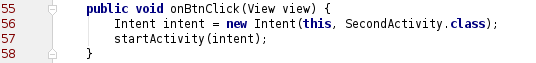
\includegraphics[scale=0.4]{chapters/ch08/images/8}
\end{center}

Code explanation:

\begin{itemize}
	\item \textit{Line 56}: Creates an intent object. Here we are explicitly mentioning the activity to be called right inside the constructor, hence making this an ``explicit intent''.
	
	\item \textit{Line 57}: Start the activity using the above intent object.
\end{itemize}

Let's build the intent a bit differently this time. Replace the code inside the button listener with the following:

\begin{center}
	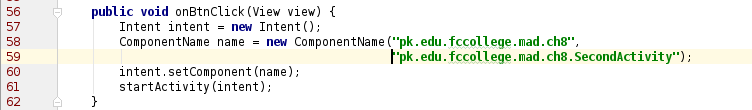
\includegraphics[scale=0.4]{chapters/ch09/images/17}
\end{center}

\begin{itemize}
	\item \textit{Line 57}: We are creating an intent object but this time with an empty constructor. We will manually provide the activity name to be called.
	
	\item \textit{Line 58-59}: Specify name of the component (this field is described in section \ref{ALI:anatomyOfIntent}). In the constructor first we give complete package name of the project. Then in the second parameter we give the ``fully qualified'' name of the activity that we want to start.
	
	\item \textit{Line 60}: Set the component name as above.
	
	\item \textit{Line 61}: Finally start the activity using above intent.
\end{itemize}

If you run this on a device and click the button on the main activity, our \texttt{SecondActivity} opens up as expected. \\

What if I told you that you can even run ANY activity of ANY app installed on your device as long as you know its exact package id and name. Suppose that you created a simple project named ``Testing Intents'' having package name ``\texttt{pk.edu.fccollege.mad.testingintents}''. This project contains just one activity called ``\texttt{MainActivity}''. Suppose that you build this project and it is already installed on your device:

\begin{center}
	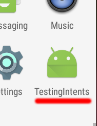
\includegraphics[scale=0.4]{chapters/ch09/images/20}
\end{center}

Now from our currently open \texttt{ch8} project, modify the event listener again as follows:

\begin{center}
	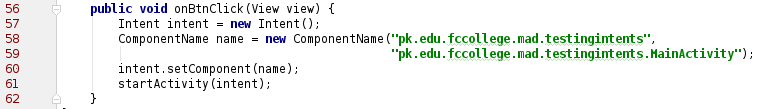
\includegraphics[scale=0.4]{chapters/ch09/images/18}
\end{center}

The only changes are made in 58 and 59. As before as a first parameter we give the package id of the app. The second parameter is the fully qualified name of the activity that we want to start. Again note that this activity belong to a \textit{different} app.

Run the project on a device and click the button on our \texttt{MainActivity}, you will see an activity opening up from an outside app. Press back button to go back to the main activity:

\begin{center}
	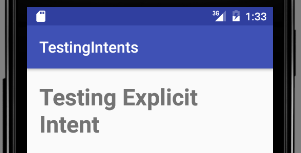
\includegraphics[scale=0.4]{chapters/ch09/images/21}
\end{center}

Let's go even further. Let's call android's default calculator. Modify the event listener as follows:

\begin{center}
	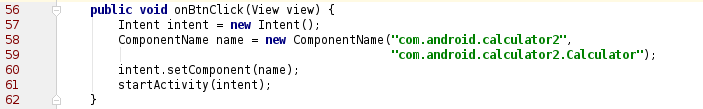
\includegraphics[scale=0.4]{chapters/ch09/images/19}
\end{center}

Again the only changes are in lines 58 and 59. First the package name of the calculator app and then the name of fully qualified activity that we want to launch from within this app. 

Run the project and you will witness a fully functional calculator inside your app. You can open a browner, keyboard, dialer, maps, ANYTHING you want! \\

Don't ask me how did I come to know the exact package name and name of the activity. If you feel like hacking, you can check out \href{http://stackoverflow.com/questions/12698814/get-launchable-activity-name-of-package-from-adb}{this cool link!} \\

If you haven't implement a feature, you can call activities of other apps ``explicitly'' to provide that feature as we've just shown. But there is a better way which we will explore in detail in section \ref{IBSR:broadcastSenders}. \\

You can read more about explicit intents \href{https://developer.android.com/guide/components/intents-filters.html#ExampleExplicit}{here}.

\subsection{Sending Data to Other Activities}

\subsection{Receiving Data from Other Activities}

\section{Broadcast Senders}
\label{IBSR:broadcastSenders}
When creating an intent if you DO NOT specify the component name then that will act as an ``Implicit Intent'' as there is no definite receiver. The android operating system will search ALL of the activities inside ALL apps installed on the device and executes the activity that best matches the job description. In case of multiple activities the android will present a dialog box (known as the app chooser) showing possible candidates for you to choose from. 

\begin{quote}
	``An activity which sends \textit{implicit intents} is called \textbf{Broadcast sender}. 
	
	An activity which receives \textit{implicit intents} is called \textbf{Broadcast receiver}''. 
\end{quote}

Suppose we need to open a website but we don't know which app on the device can help as we have no idea what is installed on the user's phone (so we can't use explicit intents). Let's first send a system wide message that we need help with our website. \\

Open up \texttt{activity\_main.xml} layout file and add a button as shown. Also attach a callback method named ``\texttt{onOpenBrowserBtnClick}'' to it:

\begin{center}
	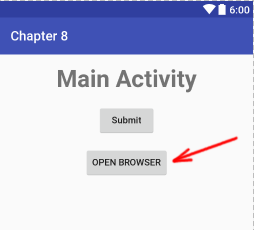
\includegraphics[scale=0.4]{chapters/ch09/images/22}
\end{center}

Inside the button callback function, add following lines of code:

\begin{center}
	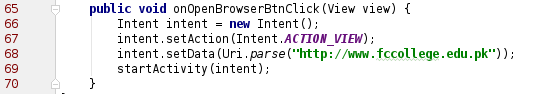
\includegraphics[scale=0.4]{chapters/ch09/images/23}
\end{center}

Let's review the code in detail:

\begin{itemize}
	\item \textit{Line 66}: Create an empty intent object.
	
	\item \textit{Line 67}: The \texttt{setAction} method accepts a string as input. An action tells what ``kind'' of message we want to broadcast. As mentioned earlier that the system searches for ALL activities and returns the best match(es). So in effect every activity will listen to this intent but only a few will respond back. Different types of broadcast receivers will be listening to different actions. For example browser will be listening to one action type,
	camera may be listening to another action type.
	
	We want to open a browser, so we need to sent a message of type or action
	``\texttt{Intent.}\href{https://developer.android.com/reference/android/content/Intent.html#ACTION_VIEW}{\texttt{ACTION\_VIEW}}''. \href{https://developer.android.com/reference/android/content/Intent.html#ACTION_VIEW}{\texttt{ACTION\_VIEW}} is just a predefined action that is related to viewing data in some way. There can be many other activities including web browsers that might listening to this action. 
	
	\texttt{ACTION\_VIEW} is actually just a string, you can look it up. Right click on \texttt{ACTION\_VIEW} and from the popup menu select ``Goto $\rightarrow$ Declaration''. That will take you to the \texttt{Intent.java} class where this string is defined:
	
	\begin{center}
		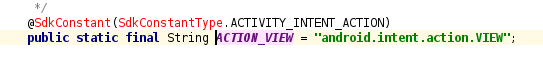
\includegraphics[scale=0.4]{chapters/ch09/images/25}
	\end{center}
	
	\item \textit{Line 68}: Set's the data as the website address that we want to launch. After receiving proper action type the broadcast receiver apps will then parse the data. If the data seem relevant then they will process it further, otherwise they will simply ignore the intent.
	
	\item \textit{Line 69}: Start the activity based on the intent above.
	
\end{itemize}

\begin{quote}
	\textit{``\textbf{Tip:} It is better to provide more fields to narrow down the search results.''}
\end{quote}

Run your app on a device. From the main activity click on ``Open Browser'' button. The website will open up in a browser activity:

\begin{center}
	
\includegraphics[scale=0.4]{chapters/ch09/images/24}
\end{center}

If you have multiple browsers installed on your device then the android operating system will show a dialog box (app chooser) of web browser candidates for you to choose from.

Great! But what if we need to send an email? We need to select a different type of action and send different type of data. Make a second button on the layout called ``Send Email'', also attach an event listener \texttt{onSendEmailBtnClick} to it:

\begin{center}
	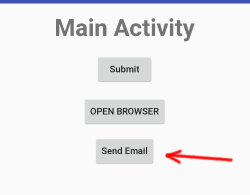
\includegraphics[scale=0.4]{chapters/ch09/images/26}
\end{center}

Open up \texttt{MainActivity.java}. Inside the \texttt{onSendEmailBtnClick} event listener type the following code:

\begin{center}
	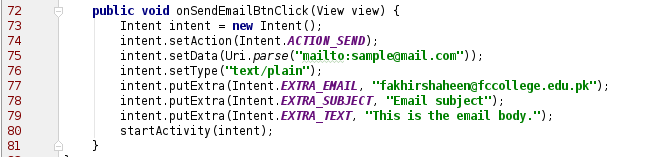
\includegraphics[scale=0.4]{chapters/ch09/images/27}
\end{center}

Line by line analysis of the code:

\begin{itemize}
	\item \textit{Line 73}: Create an empty intent object.
	
	\item \textit{Line 74}: Other apps including email clients are listening to the \href{https://developer.android.com/reference/android/content/Intent.html#ACTION_SEND}{\texttt{ACTION\_SEND}} action. Browsers are not listening to \texttt{ACTION\_SEND} because they are listening to \texttt{ACTION\_VIEW} :-)
	
	\item \textit{Line 75}: Just like the browser we set the data as the email address of our recipient.
	
	\item \textit{Line 76-79}: Depending on the type of action and broadcast receiver there can be potentially additional data that the receiving app may require. You have to check the app manual or	documentation for that.
	
	\item \textit{Line 80}: Start the activity based on the intent above.
	
\end{itemize}

As soon as you launch the app and press the ``Send Email'' button, it will show you all the apps that are listening to the \texttt{ACTIVITY\_SEND} event. Remember that \texttt{ACTIVITY\_SEND} is just a string, you can even check out its actual value. In my case it listed a few possible email clients that were installed on my device. If my custom app was listening to \texttt{ACTIVITY\_SEND} type of action then my app would've also been listed in this list:

\begin{center}
	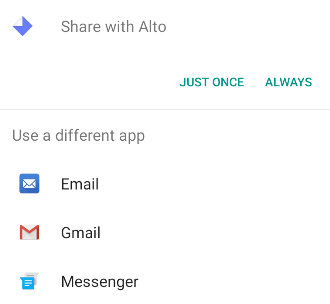
\includegraphics[scale=0.4]{chapters/ch09/images/28}
\end{center}

Chose any option and witness the email message filled with our given details. \\

Apart from sending emails, do you want to open a dialer? No problem! Create a third button:

\begin{center}
	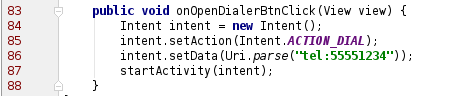
\includegraphics[scale=0.4]{chapters/ch09/images/29}
\end{center}

\begin{itemize}
	\item \textit{Line 84}: Create empty intent object.
	
	\item \textit{Line 85}: Set the action to \href{https://developer.android.com/reference/android/content/Intent.html#ACTION_DIAL}{\texttt{ACTION\_DIAL}}. Ofcourse browser, email client or any other non-related app won't be listening to this action.
	
	\item \textit{Line 86}: Set the phone number as data.
	
	\item \textit{Line 87}: Broadcast the intent.
	
\end{itemize}

Run your app on a device and check if dialer is properly opening up when you click the ``open dialer'' button. \\

Not enough? Need more stuff? Want to display a map? Open a camera? Play with calendar events? Check out the following android reference to do all of this and more fancy stuff:

\url{http://developer.android.com/training/basics/intents/sending.html} \\

Now we will see how to make our app a broadcast receiver so that our app can respond to other intents just like the web browser or email clients we just saw above!

\section{Broadcast Receivers}

\subsection{Create New Project}
\begin{enumerate}
	\item Create a new project having name ``\texttt{Ch9Reveiver}''
	\item Select minimum API 16 : Android 4.1 (Jelly Bean).
	\item Choose blank activity.
	\item Accept default values for activity and click finish. \\
\end{enumerate}

This looks like the usual app that we've made a million times. We will be extending this app to be a broadcast receiver as well. 

Let's add a receiver class. Go to the project panel, under java, right click the bundle id: 

\begin{center}
	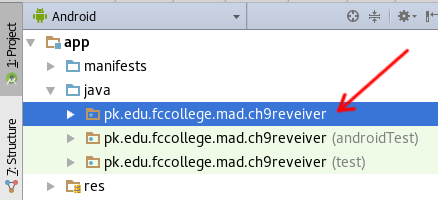
\includegraphics[scale=0.4]{chapters/ch09/images/30}
\end{center}

From the popup menu select ``New'' $\rightarrow$ ``Other'' $\rightarrow$ ``Broadcast receiver''. A component configure dialog box will open up. Accept default values and hit finish:

\begin{center}
	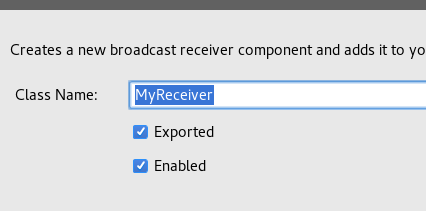
\includegraphics[scale=0.4]{chapters/ch09/images/31}
\end{center}

This will create a new java file named ``\texttt{MyReceiver.java}''. Open up ``\texttt{MyReceiver.java}'', the code should look like below:

\begin{center}
	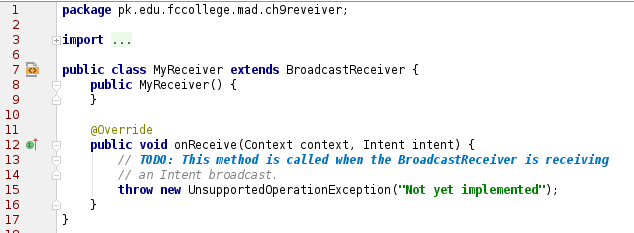
\includegraphics[scale=0.4]{chapters/ch09/images/32}
\end{center}

Code explanation:

\begin{itemize}
	\item \textit{Line 7}: \texttt{MyReceiver} class is inheriting the ``\href{https://developer.android.com/reference/android/content/BroadcastReceiver.html}{\texttt{BroadcastReceiver}}'' base class.
	
	\item \textit{Line 8}: The constructor, we will leave it empty.
	
	\item \textit{Line 12}: This is the meat of the activity. \texttt{OnReceive} callback method is called as soon as this activity receives an intent or message that it is interested in.
	
	\item \textit{Line 15}: We will delete this line soon.

\end{itemize}

Let's add a toast inside \texttt{onReceive}. Delete ``\texttt{throw new ...}'' (line 15), replace it with the following code:

\begin{center}
	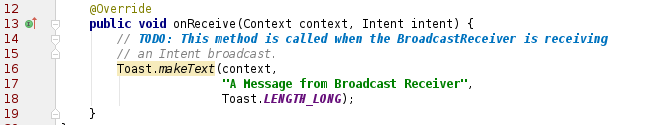
\includegraphics[scale=0.4]{chapters/ch09/images/33}
\end{center}

\subsection{Intent Filters}
We are almost done. This listener is listening to all of the events in the universe. We don't want that. We don't want to listen to the browser related \texttt{ACTION\_VIEW} actions. We want to ``filter'' out the intents that we are interested in, hence we are going to add an intent filter in our manifest file.

\begin{quote}
	``\href{https://developer.android.com/guide/components/intents-filters.html#Receiving}{\textbf{Intent Filters:}} are conditions that dictate what kind of intents the receiver can receive. Intent filters must be defined in the \texttt{AndroidManifest} file before a receiver can start receiving intents.''
\end{quote}

Open up \texttt{AndroidManifest.xml}. Here you need to add an ``intent filter''. As mentioned above intent filter tells your app to only listen to intents/messages that have a special keyword or passcode or action string (as we saw in the previous activity). This can be ANY string that we want. Add \texttt{<intent-filter>} tags INSIDE the \texttt{<receiver>} tags and specify the action and category strings as follows (lines 23-26):

\begin{center}
	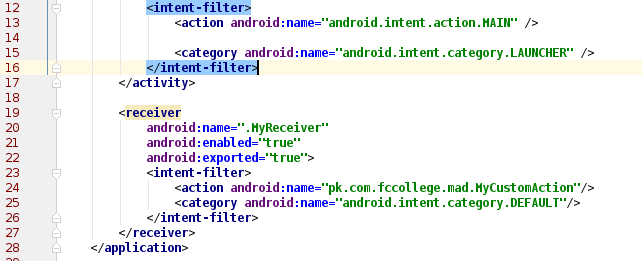
\includegraphics[scale=0.4]{chapters/ch09/images/34}
\end{center}

You can define three things in an intent filter to filter out the intents:

\begin{enumerate}
	\item \textit{action}: You can specify any string here. We specified \texttt{pk.com.fccollege.mad.MyCustomAction} but you can give any \href{https://developer.android.com/reference/android/content/Intent.html#constants}{default action strings} provided by android. 
	
	Your app will only react to the intents when the broadcast senders specify your custom action given in the intent filter.
	
	\item \textit{category}: What kind of receiver is the sender requesting? Is it a browser? email client? dialler etc. More information about default categories can be found \href{https://developer.android.com/reference/android/content/Intent.html#CATEGORY_APP_BROWSER}{here}.
	
	\item \textit{data}: What kind of data is provided with the the intent. \\
	
\end{enumerate}

Here we are using action tag and the category tag. You should always set the category tag to any value, even if it is \texttt{DEFAULT}. \\

Run the app to install it on the device. Close this project and open up the previous \texttt{chapter 8} project. Create a new button named ``Custom Intent'':

\begin{center}
	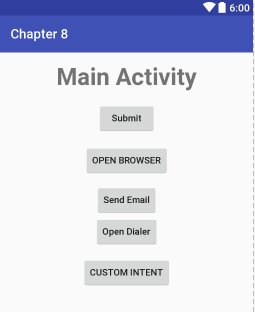
\includegraphics[scale=0.4]{chapters/ch09/images/35}
\end{center}

Hook it to listener named ``\texttt{onCustomIntentBtnClick}'':

\begin{center}
	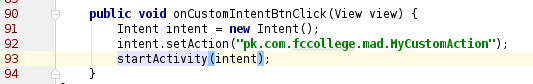
\includegraphics[scale=0.4]{chapters/ch09/images/36}
\end{center}

Explanation: